\documentclass[parskip, 12pt, DIV=16, openany]{scrartcl}

\usepackage{german}
\usepackage[utf8]{inputenc}
\usepackage{amsmath}
\usepackage{enumerate}
\usepackage{hyperref}
\usepackage{graphicx}
\usepackage[german]{cleveref}
\usepackage{booktabs}
\usepackage{pdfpages}
\usepackage{afterpage}
\usepackage{float}
%\usepackage[per-mode=fraction, exponent-product=\cdot, output-decimal-marker={,}, uncertainty-mode=separate]{siunitx}
\usepackage[per-mode=fraction, exponent-product=\cdot, output-decimal-marker={,}]{siunitx}

%\usepackage{txfonts}
\usepackage{tikz}

%\usepackage[T1]{fontenc}
%\usepackage{lmodern}

\DeclareUnicodeCharacter{0394}{\ensuremath{\Delta}}

\newcommand{\Z}{\mathbb Z}

%\renewcommand{\thefootnote}{\fnsymbol{footnote}}
\renewcommand{\thefootnote}{\textit\arabic{footnote}}


\newcommand{\DefVal}[2]{%
  \expandafter\newcommand\csname val-#1\endcsname{#2}%
}
\newcommand{\Val}[1]{\csname val-#1\endcsname}
\DefVal{_}{0.7021125760141528}
\DefVal{c1}{12.211599818576055}
\DefVal{dc1}{0.04105725358249311}
\DefVal{X2_1}{0.3882876282488006}
\DefVal{dof_1}{18}
\DefVal{R1}{81.88935232538647}
\DefVal{dR1}{0.2753244418487307}
\DefVal{index}{10}
\DefVal{a2q}{16.185711504480224}
\DefVal{b2q}{-0.08482659918456946}
\DefVal{da2q}{0.06734309521650214}
\DefVal{db2q}{0.0011768583504398933}
\DefVal{X2_2q}{3155.733607790688}
\DefVal{dof_2q}{24}
\DefVal{a2a}{6.128593619547221}
\DefVal{b2a}{22.036837779574704}
\DefVal{da2a}{0.07659683834498186}
\DefVal{db2a}{0.24332252384572234}
\DefVal{X2_2a}{148.82713602429988}
\DefVal{dof_2a}{24}
\DefVal{R1_lit}{82.5}
\DefVal{dR1_lit}{0.8250000000000001}
\DefVal{t}{0.7021125760141528}
\DefVal{_20}{0.7021125760141528}

\newcommand{\SIp}[3]{\SI[round-mode=places,round-precision=#1]{\Val{#2}}{#3}}
\newcommand{\SIu}[3]{\SI[round-mode=uncertainty,round-precision=2]{\Val{#1}\pm\Val{#2}}{#3}}


%\title{Versuch 45

\begin{document}
\begin{center}

\vspace{2cm}

\large
Universität Freiburg \\
Physiklabor für Anfänger*innen Teil 2\\
Ferienpraktikum im WS 2022/23

\vspace{2cm}
\vspace{2cm}
{\sectfont
 \Huge Versuch 45\\Strom-Spannungs-Kennlinien\par
}
\vspace{2cm}

{\Large
Müller, André\\
Kopp, Manuel\\
Breitner, Joachim\\
(Gruppe 121)\\
}

\end{center}
\vspace{2cm}
\vspace{2cm}
\vspace{2cm}
\vspace{2cm}

{\large
Durchführung: 23. Februar 2023\\
Protokollerstellung: \today\\
Assistent: Tim Gitzinger
}

\pagebreak
\section{Ziel des Versuchs}

Wir messen Strom-Spannungs-Kennlinien für verschiedene zweipolige elektrische Bauteile.

\section{Versuchsdurchführung}

Wir untersuchen einen Tantal-Draht. Mittels einer Messschraube ermittelten wir dessen Durchmesser von $d = \SIu{d}{dd}{\mm}$.

Wir ermitteln den spezifischen Widerstand des Drahtes, in dem wir durch den Draht einen Strom der Stärke $I$ fließen lassen, und dabei auf einem Abschnitt der Länge $l$ die Spannungsdifferenz $U$ messen.

\begin{figure}
\centering
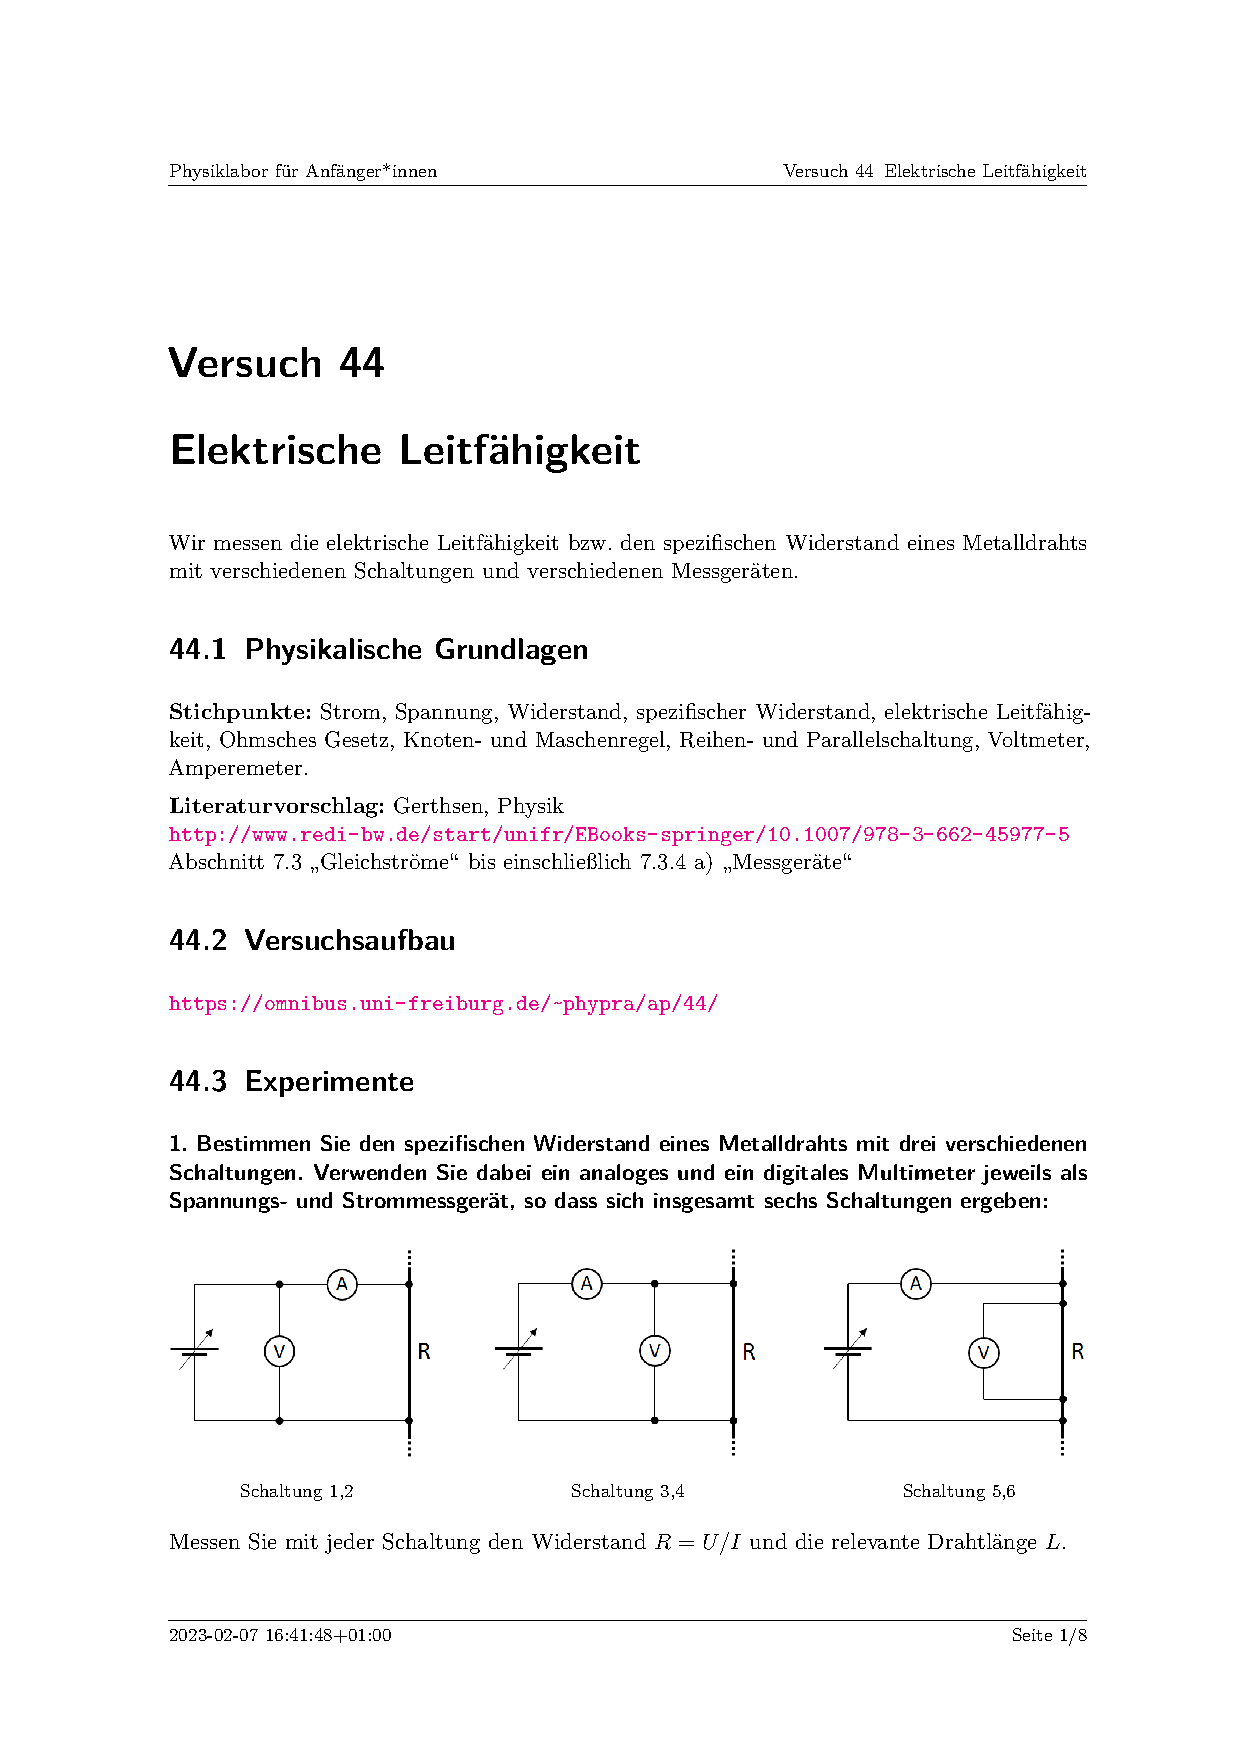
\includegraphics[page=1,trim=3cm 4cm 3cm 21cm,clip]{Versuch 44.pdf}
\caption{Schaltungsaufbau (aus der Versuchsbeschreibung)}\label{fig:schaltungen}
\end{figure}

Im ersten Versuchsteil verwendeten wir dazu verschiedene Schaltungen (siehe \cref{fig:schaltungen}). Bei den Schaltungen 1, 3 und 5 wurde ein digitales Multimeter (Uni-T 51) zur Spannungsmessung verwendet und ein analoges (PeakTech 3260) zur Stromstärkemessung, bei den Schaltungen 2, 4 und 6 wurden das jeweils andere Gerät verwendet. Die Länge des Drahts wurde mit einem Metermaß bestimmt. Das Labornetzteil haben wir so eingestellt, dass die Leistungsaufnahme des Drahtes im Bereich von \SI{1}{\W} liegt.

Die Messergebnisse der sechs Schaltungen sind in \cref{tab1} aufgeführt. Die Ungenauigkeiten haben auf Basis der Datenblätter in der Versuchsbeschreibung berechnet.

Bei den ersten Messungen ist uns der Draht mehrfach verrutscht, daher die Streichung in den Versuchsnotizen.

\begin{table}
\begin{center}

\begingroup
\sisetup{round-mode=uncertainty,round-precision=2}
\begin{tabular}{SSS}
\toprule
{$U$ (\unit{\V})} & {$I$ (\unit{\mA})} & {$R$ (\unit{\ohm})} \\
\midrule
0.085\pm0.001425 & 1.03\pm0.01645 & 82.5242718446602\pm1.9107963173389984  \\
0.215\pm0.002075 & 2.62\pm0.0403 & 82.06106870229007\pm1.4901282445500277  \\
0.352\pm0.00276 & 4.29\pm0.06535 & 82.05128205128206\pm1.4057547050767423  \\
0.424\pm0.00312 & 5.18\pm0.07869999999999999 & 81.85328185328186\pm1.3817846378985987  \\
0.502\pm0.00351 & 6.13\pm0.09294999999999999 & 81.89233278955955\pm1.3674035526704096  \\
0.602\pm0.00401 & 7.36\pm0.1114 & 81.79347826086956\pm1.3526010073176424  \\
0.703\pm0.004515 & 8.59\pm0.12985 & 81.83934807916181\pm1.3441453878077414  \\
0.859\pm0.005295 & 10.5\pm0.1585 & 81.80952380952381\pm1.3339290309657137  \\
0.968\pm0.00584 & 11.83\pm0.17845 & 81.82586644125107\pm1.3293640343097142  \\
1.06\pm0.0063 & 12.96\pm0.19540000000000002 & 81.79012345679013\pm1.325516709988082  \\
-0.156\pm0.00022000000000000003 & -1.9\pm0.027499999999999997 & 82.10526315789474\pm1.1939933511625174  \\
-0.405\pm0.0010250000000000003 & -4.96\pm0.07339999999999999 & 81.65322580645163\pm1.2258799080636815  \\
-0.553\pm0.001765 & -6.76\pm0.10039999999999999 & 81.80473372781066\pm1.2427074615075924  \\
-0.604\pm0.00202 & -7.38\pm0.10969999999999999 & 81.84281842818427\pm1.2469637361303585  \\
-0.704\pm0.0025199999999999997 & -8.6\pm0.128 & 81.86046511627906\pm1.2531291720770055  \\
-0.747\pm0.002735 & -9.12\pm0.13579999999999998 & 81.90789473684211\pm1.2559655039773003  \\
-0.793\pm0.0029650000000000006 & -9.69\pm0.14434999999999998 & 81.83694530443756\pm1.2569220811332358  \\
-0.876\pm0.00338 & -10.71\pm0.15965000000000001 & 81.79271708683473\pm1.2594357869337793  \\
-0.94\pm0.0037 & -11.49\pm0.17135 & 81.81026979982593\pm1.2618157927322506  \\
-1.551\pm0.006755 & -18.96\pm0.2834 & 81.80379746835442\pm1.2735901491512711  \\

\bottomrule
\end{tabular}
\endgroup

\end{center}
\caption{Verschiedene Schaltungen}
\label{tab1}
\end{table}

Für den zweiten Versuchsteil, in dem wir die Länge des vermessenen Drahtstücks variieren sollen, wählten wir Schaltung 5 aus, aus folgenden Gründen
\begin{itemize}
\item Schaltung 1  und 2 disqualifizieren sich dadurch, dass die Spannungsmessung auch den Amperemeter, und damit dessen Widerstand, erfasst.
\item Schaltung 5 und 6 bieten sich dadurch an, dass die Spannungsmessung direkt mit eigenen Krokodilklemmen direkt am Draht erfolgt,
\item Bei Schaltung 5 wird das digitale Multimeter zur Spannungsmessung verwendet. Da wir erwarten, dass die Spannung mit der Drahtlänge kleiner wird, die Stromstärke aber gleich bleibt, bietet sich an, hier das genauere Gerät zu nehmen.
\end{itemize}

\begin{table}
\begin{center}

\begingroup
\sisetup{round-mode=uncertainty,round-precision=2}
\begin{tabular}{SSS}
\toprule
{$U$ (\unit{\V})} & {$I$ (\unit{\mA})} & {$R$ (\unit{\ohm})} \\
\midrule
0.47\pm0.01235 & 16.4\pm0.346 & 28.658536585365855\pm0.9657401960053867  \\
0.95\pm0.01475 & 23.3\pm0.4495 & 40.7725321888412\pm1.00967953484316  \\
1.22\pm0.0161 & 26.8\pm0.502 & 45.52238805970149\pm1.0430655095557169  \\
1.54\pm0.0177 & 30.7\pm0.5605 & 50.1628664495114\pm1.0822058651837434  \\
1.84\pm0.019200000000000002 & 33.9\pm0.6084999999999999 & 54.277286135693224\pm1.126932789788907  \\
2.05\pm0.020249999999999997 & 36.0\pm0.64 & 56.944444444444436\pm1.1581234924717514  \\
2.47\pm0.022350000000000002 & 40.2\pm0.703 & 61.44278606965174\pm1.2098015700314673  \\
2.97\pm0.024850000000000004 & 44.8\pm0.7719999999999999 & 66.29464285714288\pm1.2699421802701198  \\
3.82\pm0.0291 & 52.4\pm0.8859999999999999 & 72.90076335877862\pm1.3519598991210533  \\
4.44\pm0.0322 & 57.2\pm0.958 & 77.62237762237763\pm1.4166862231362554  \\
5.11\pm0.035550000000000005 & 62.3\pm1.0345 & 82.02247191011237\pm1.47669990498443  \\
9.84\pm0.0592 & 92.2\pm1.483 & 106.72451193058568\pm1.832773122203632  \\
6.23\pm0.041150000000000006 & 70.0\pm1.1500000000000001 & 89.00000000000001\pm1.5758926851477044  \\
6.96\pm0.0448 & 74.9\pm1.2235 & 92.92389853137516\pm1.6315173919886545  \\
7.92\pm0.049600000000000005 & 80.9\pm1.3135000000000001 & 97.89864029666253\pm1.7036367240548855  \\
9.05\pm0.05525000000000001 & 87.7\pm1.4155 & 103.19270239452679\pm1.7807197324259318  \\
-1.07\pm0.00465 & -24.6\pm0.269 & 43.49593495934959\pm0.5118110774054557  \\
-2.04\pm0.00020000000000000052 & -35.9\pm0.4385 & 56.82451253481894\pm0.69410449528584  \\
-3.16\pm0.005800000000000001 & -46.5\pm0.5975 & 67.95698924731184\pm0.8820742185078392  \\
-4.08\pm0.010400000000000001 & -54.2\pm0.7130000000000001 & 75.27675276752767\pm1.008683321126557  \\
-4.97\pm0.01485 & -61.1\pm0.8165 & 81.34206219312603\pm1.1138414676404944  \\
-6.0\pm0.019999999999999997 & -68.5\pm0.9274999999999999 & 87.59124087591242\pm1.2214084709417883  \\
-7.08\pm0.0254 & -75.5\pm1.0325 & 93.77483443708608\pm1.3258112556801032  \\
-7.97\pm0.029849999999999995 & -81.4\pm1.121 & 97.91154791154791\pm1.3973642077298354  \\
-8.97\pm0.03485 & -87.2\pm1.208 & 102.86697247706422\pm1.4800195390254645  \\
-9.84\pm0.0392 & -92.3\pm1.2844999999999998 & 106.60888407367281\pm1.5432212503806522  \\

\bottomrule
\end{tabular}
\endgroup

\end{center}
\caption{Schaltung 2, verschiedene Längen, $I = \SIu{I}{dI}{\A}$}
\label{tab2}
\end{table}

Wir wählten daher Schaltung 5. Wir stellten das Netzteil so ein, dass (laut analogem Multimeter) stets $I = \SI1{\A}$ Strom floss. Dies erforderte zum Teil nachjustieren.
Wir machten 12 Messungen, deren Werte in \cref{tab2} aufgeführt sind.


\section{Auswertung}

\subsection{Fehleranalyse und -beiträge}

Aus $d$, $l$, $I$ und $U$ können wir per
\[
\varrho = \frac{U \pi (\frac d2)^2}{I l}
\]
den spezifischen Widerstand berechnen. Siehe \cref{tab1} und \cref{tab2} für Ergebnisse der jeweiligen Messungen. Die Unsicherheit wurde dabei über die Gauß'sche Fehlerfortpflanzung berechnet.

Wie oben besprochen erschien uns Schaltung 5 von den Schaltungen im ersten Versuchsteil die sinnvollste; für diese berechnen wir die jeweiligen Beiträge der Unsicherheiten der Messwerte:
\begin{center}
\begin{tabular}{SSSSSS}
\toprule
{$\varrho$ ($\mathrm{\mu\Omega m}$)} & {$|\frac{\partial \varrho}{\partial U}|\Delta U$} & {$|\frac{\partial \varrho}{\partial I}|\Delta I$} & {$|\frac{\partial \varrho}{\partial l}|\Delta l$} & {$|\frac{\partial \varrho}{\partial d}|\Delta d$} & {$\Delta \varrho$} \\
\midrule
0.1426 & 0.0013 & 0.0029 & 0.0020 & 0.0114 & 0.0120 \\
\bottomrule
\end{tabular}

\end{center}

Wir sehen dass die Unsicherheit des Drahtdurchmessers (der ja quadratisch in den spezifischen Widerstand eingeht) mit Abstand den größten Beitrag liefert.

\subsection{Zusammenhang $l$ und $U$}

\begin{figure}
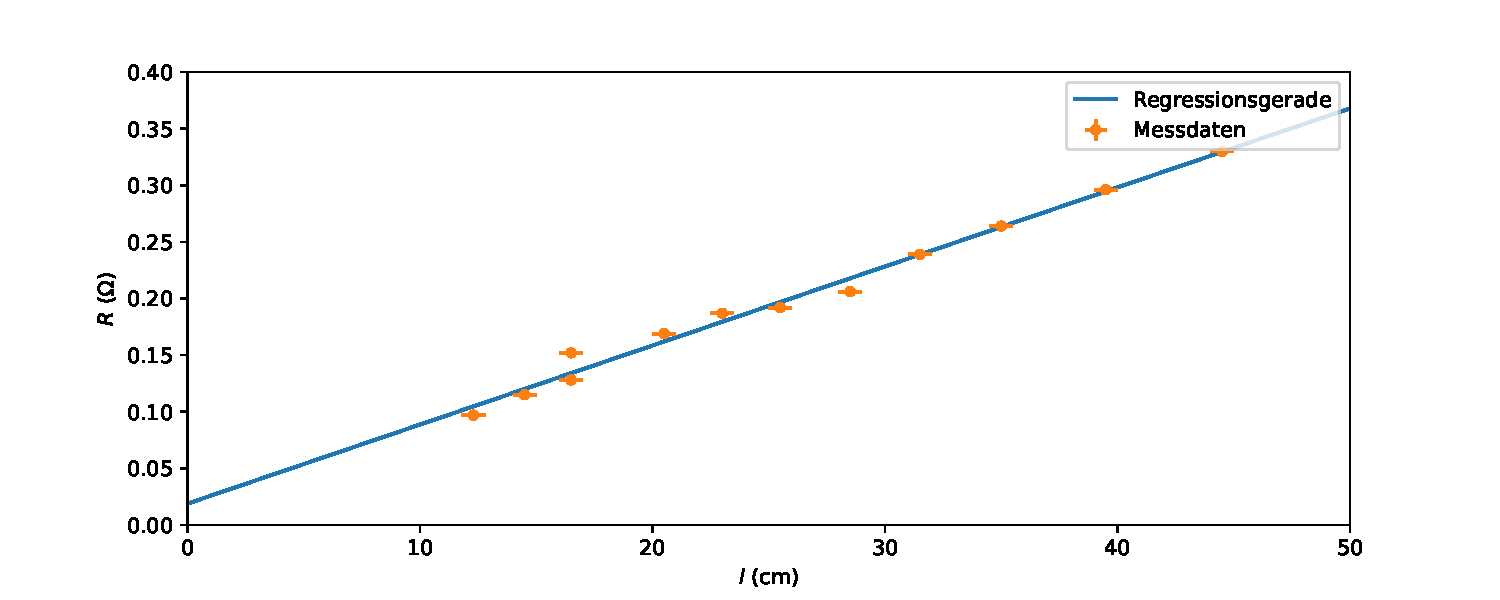
\includegraphics[width=\linewidth]{plot1}%
\vspace*{-.9cm}\\
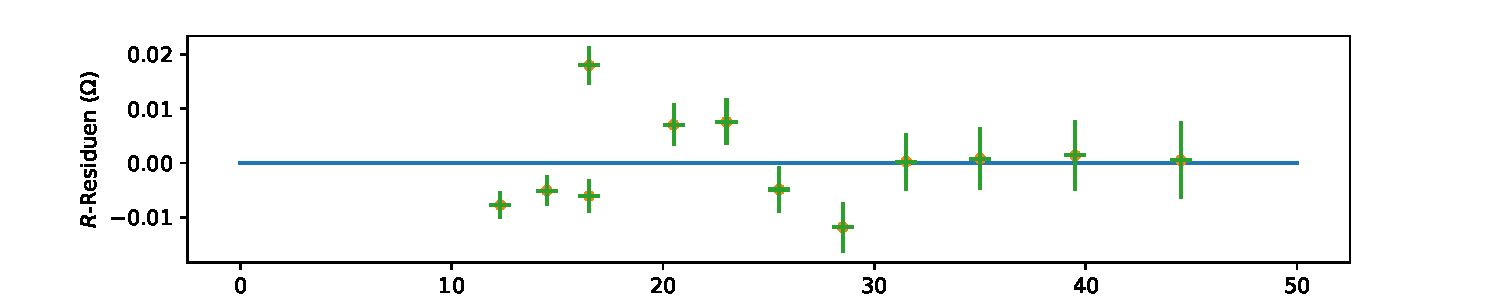
\includegraphics[width=\linewidth]{plot1residuen}
\caption{Gemessener Widerstand in Abhängigkeit der vermessenen Drahtlänge}\label{fig:R}
\end{figure}


Weiter untersuchen wir den Zusammenhang zwischen Drahtlänge und gemessener Spannung im zweiten Versuchsteil. Dazu berechnen wir den gemessenen Widerstand $R = \frac{U}{I}$, und plotten ihn in \cref{fig:R} über die Länge.

Wie die eingezeichnete Ausgleichsgerade (per ungewichteter linearer Regression ermittelt) und das zugehörige Residuendiagramm zeigen, sind die Messwerte mit dem erwarteten linearen Zusammenhang zwischen Spannungsdifferenz und Drahtlänge gut verträglich.

\subsection{Literaturvergleich}

Der Literaturwert\footnote{\url{https://en.wikipedia.org/wiki/Tantalum}, 22. Februar 2023} für den spezifischen Widerstand von Tantal bei \SI{20}{\celsius} ist $\varrho_{\text{lit}} = \SIp{3}{rho_lit}{\micro\ohm\meter}$. Dieser ist mit $t = \SIp{2}{t}{}$ mit dem im Versuchsaufbau 5 ermittelten Wert $\varrho = \SIu{rho}{drho}{\micro\ohm\meter}$ gut verträglich.

Eine alternative Bestimmung von $\varrho$ ist, die im zweiten Versuchsteil für jede Messung erhaltenen Werte entsprechend ihrer Unsicherheiten gewichtet zu mitteln. Dies ergibt einen Wert von $\varrho_2 = \SIu{rho2}{drho2}{\micro\ohm\meter}$, was allerdings signifikant ($t = \SIp{2}{t2}{}$) vom Literaturwert abweicht.

\section{Diskussion}

\subsection{Vergleich der Schaltungen}

Von den drei Schaltplänen sind nicht alle gleich gut geeignet, den spezifischen Widerstand des Tantal-Drahtes zu ermitteln:  Bei Schaltung 1 und 2 wird auch der Widerstand des Amperemeters vom Spannungsmesser erfasst, was die deutlich zu großen Werte erklärt.

Aber auch bei Schaltung 3 und 4 misst das Spannungsmessgerät auch noch den Widerstand der Leitung zwischen Draht und der Stelle, an der das Spannungsmessgerät an den Stromkreis angeschlossen wird (in unserem Fall war das eine Krokodilklemme mit Bananenstecker). Diese (dicken) Leitungen haben vermutlich einen geringen Widerstand, aber scheinbar genug um die Diskrepanz in \cref{tab1} hervorzurufen.

Daher ist Schaltung 5 und 6 deutlich sinnvoller. Die Leitung vom Messgerät zum Draht selbst ist dabei kein Problem, da dort kein Strom fließt, sobald sich das Spannungspotential ausgeglichen hat. Somit beeinflusst der Widerstand dieser Kabel unsere Messung nicht.

\subsection{Unterschätzung der Messwerte}

Die große Abweichung der ermittelten Werte für den spezifischen Widerstand vom Literaturwert verlangen nach einer Erklärung. Eine mögliche Erklärung ist, dass wir die Unsicherheiten unserer analogen Spannungs- und Stromstärkemessungen unterschätzen: Hier haben wir oben lediglich die im Datenblatt angegebene Unsicherheit von 2\% verwendet. Eventuell ist dies aber nicht groß genug um auch die Unsicherheit beim Ablesen der analogen Anzeige selbst abzudecken.

\subsection{Verbesserung der Messung}

Aufgrund des großen Einflusses der Drahtdurchmessermessung auf das Ergebnis ist hier zuerst anzusetzen, und hier eine genauere Messung zu versuchen – eventuell mittels dem von uns nicht genutzten Mikroskop.

Der nächstgrößte Beitrag zur Ungenauigkeit stammt von der Messung der Drahtlänge. Der Draht war schon leicht verbogen, was eine präzise Messung erschwerte. Hier könnte man den Aufbau verbessern, in dem man den Draht stabil und gut gespannt zwischen zwei (isolierten!) Halterungen einspannt, so dass sich die Position der Krokodilklemmen gut mit einem Maßstab messen lässt. Eine optische Bank mit Maßstab auf der Halterung könnte hier helfen.

Bei der zweiten Versuchsreihe haben wir meist, aber nicht immer, den Stromfluss präzise bei \SI{1}{\A} gehalten. Mehr Sorgfalt hier hätte vielleicht den Ausreißer in \cref{fig:R} vermieden.

Der spezifische Widerstand ist prinzipiell temperaturabhängig, so dass eine Überwachung der Drahttemperatur die Messung verbessern müsste. Auch wenn wir hin und wieder händisch geprüft haben, ob der Draht merklich warm wird, können wir damit keine leichte aber messwertrelevante Erwärmung ausschließen. Bei einem Stromfluss von \SI{1}{\A} ist eine Aufheizung des dünnen Drahtes nicht unplausibel, und könnte die signifikanten Abweichungen beim zweiten Versuchsteil erklären.

Eine Faustregel\footnote{\url{https://de.wikipedia.org/wiki/Elektrische_Leitf\%C3\%A4higkeit\#Temperaturabh\%C3\%A4ngigkeit}, 23. Februar 2023} besagt, dass jedes Kelvin Temperaturerhöhung den Widerstand um \SI{0,5}{\percent} erhöht. Die Veränderung des spezifischen Widerstandes im Verlauf der zweiten Messreihe von etwa \SIp{1}{incr}{\percent} könnte also durch eine Erwärmung von \SIp{0}{incrT}{\kelvin} erklärt werden. Bei einer Leistung von etwa \SIp{2}{power}{\W}, einer Dichte von \SIp{2}{dens}{\g\per\cm\cubed}, einer spezifischen Wärmekapazität von \SIp{0}{wkap}{\J\per\kg\per\K} bräuchte es um die \SIp{2}{mass}{\g} Draht zu erhitzen lediglich \SIp{1}{time}{\s} (wobei wir die Kühlung durch die Luft in dieser Überschlagsrechnung ignorieren) -- es ist also sehr plausibel dass wir zu viel Energie durch den Draht geschickt haben.

\subsection{Korrelation von $U$ und $I$}

Unserer Betreuer wies uns darauf hin, dass die Werte von $U$ und $I$ korreliert sind. Zum einen ist das erwünscht, da der gesuchte Widerstand gerade die Proportionalitätskontante ist. Zum anderen schränkt es die Anwendbarkeit der Gauß'schen Fehlerfortpflanzung ein, die ja von \emph{unabhängigen} normalverteilten Eingangsvariablen ausgeht. In unserem Fall sollte der Effekt allerdings vernachlässigbar sein, vor allem da ja die Ungenauigkeiten der (unabhängigen) Längen- und Durchmessermessungen dominieren.

\appendix
\section{Versuchsnotizen}\label{sec:labnotes}
\begin{center}
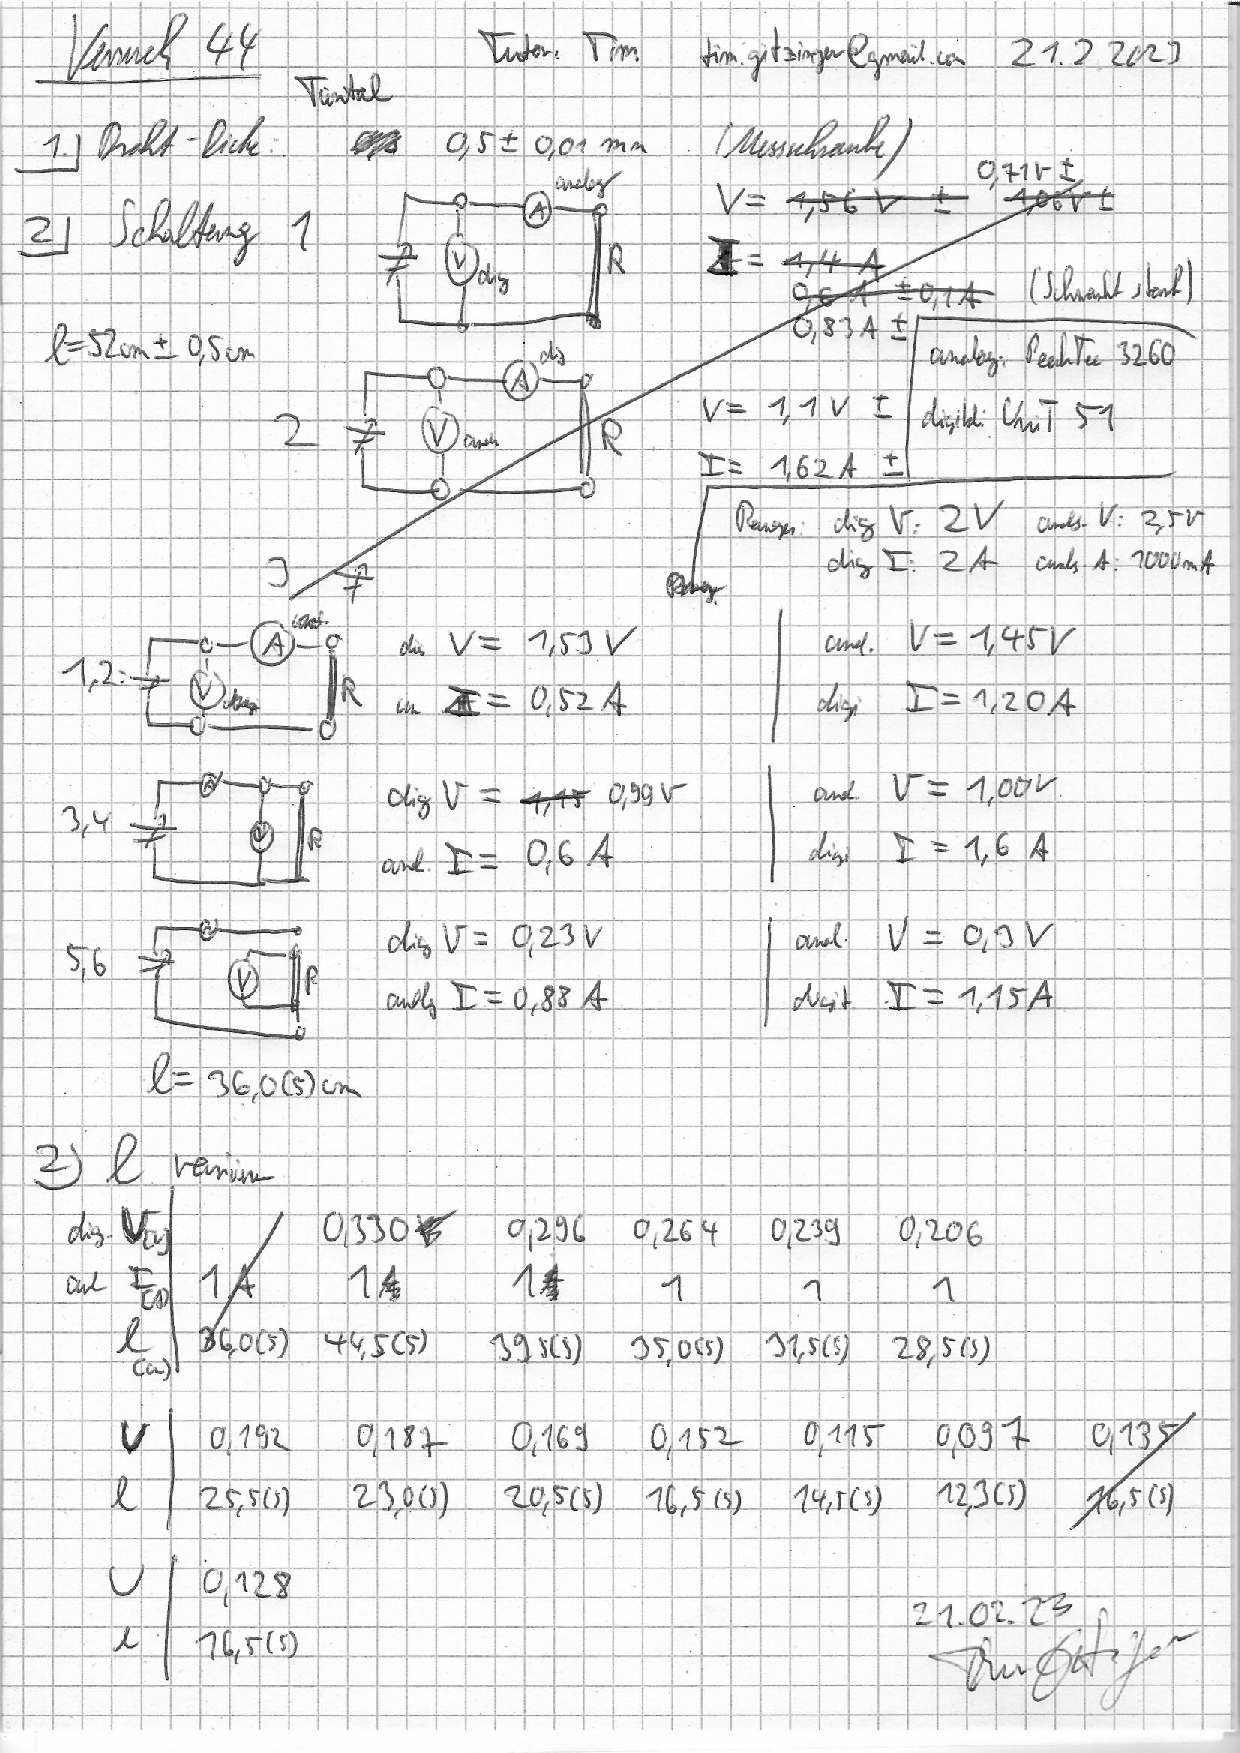
\includegraphics[page=1,scale=0.75]{labnotes.pdf}
\end{center}

\pagestyle{empty}

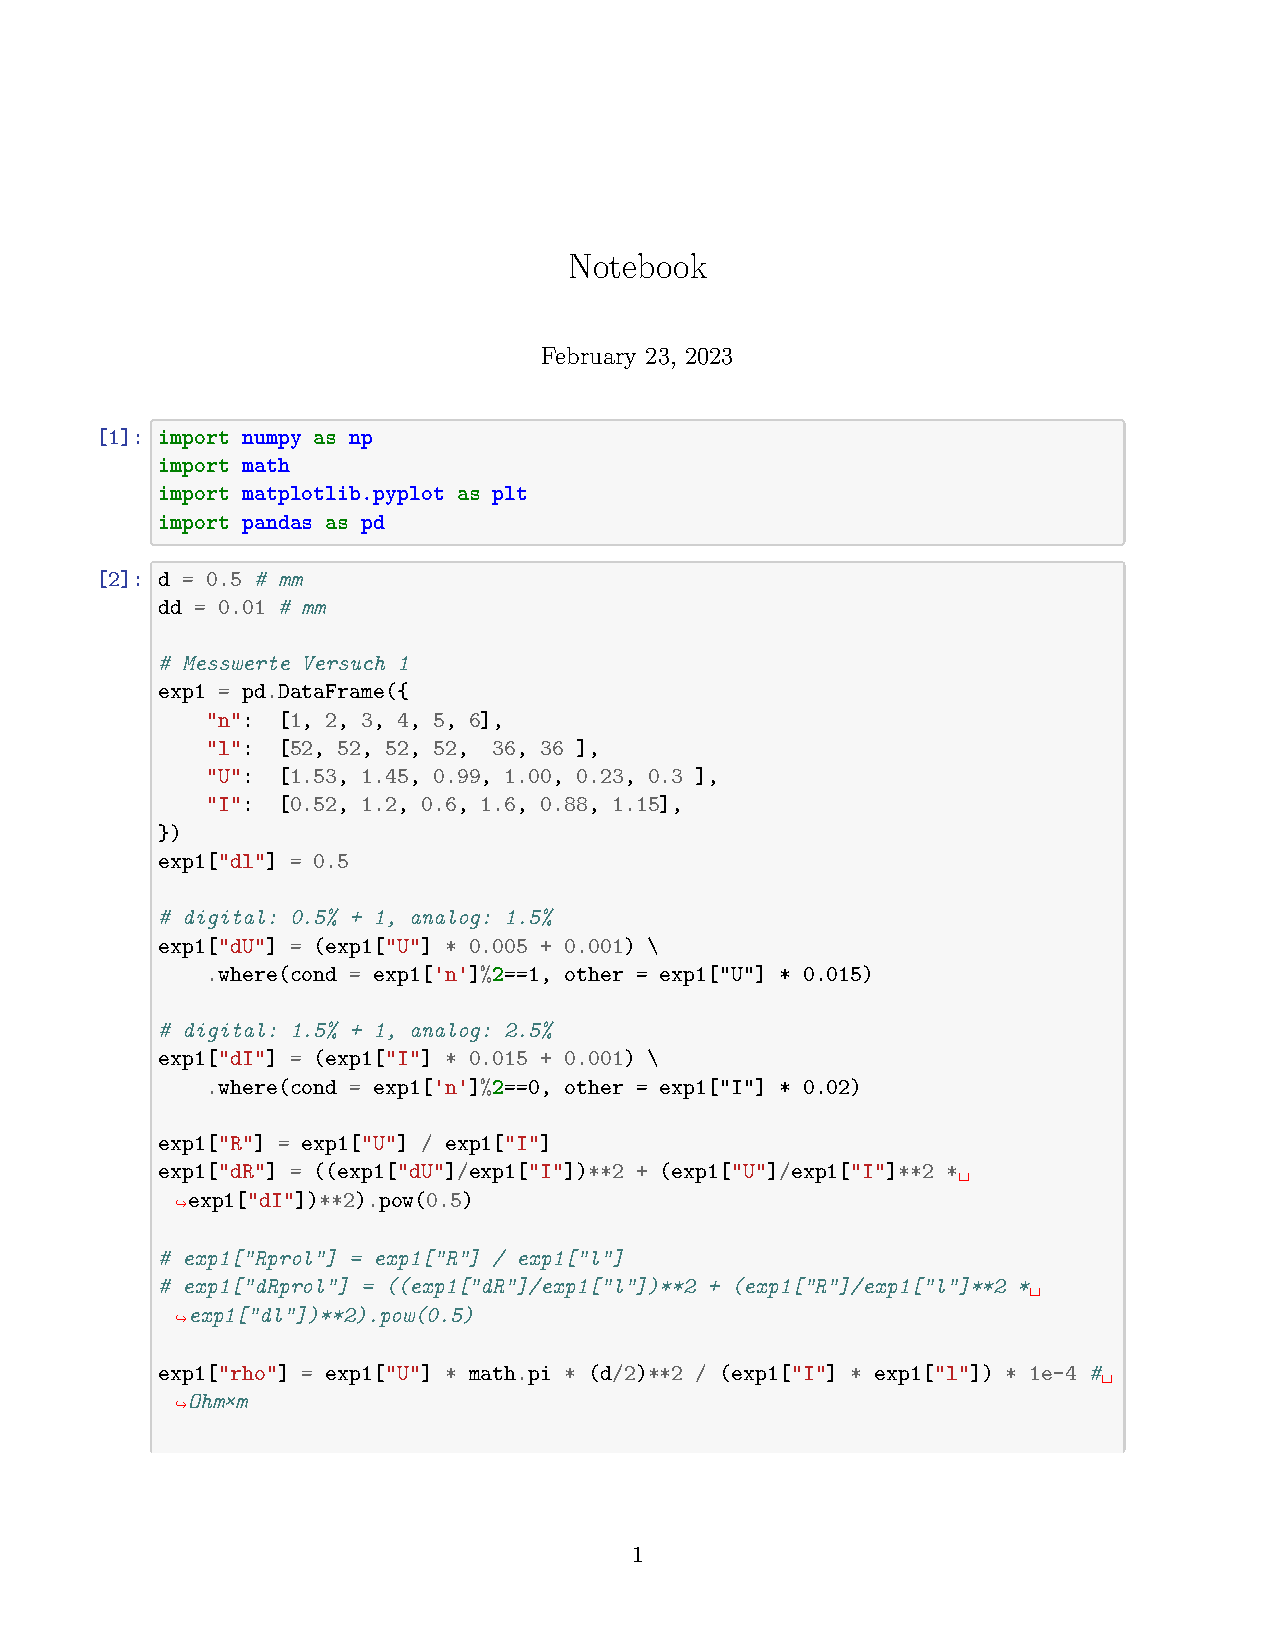
\includepdf[pages=1,scale=1,pagecommand={\section{Jupyter-Quellen}}]{Notebook.pdf}
\includepdf[pages=2-,scale=1,pagecommand={},linktodoc=true]{Notebook.pdf}

\end{document}
